% DUNE experiment
% Target length: 20 pages

\graphicspath{{DUNE/Figs/}}

\chapter{The Deep Underground Neutrino Experiment}\label{chap:DUNE}

The Deep Underground Neutrino Experiment (DUNE) experiment \cite{DUNECDR1,DUNECDR2,DUNECDR3,DUNECDR4} is a future long-baseline neutrino experiment with a diverse program of other physics hosted by Fermilab, IL, U.S..  The far detector will be at the Sanford Underground Research Facility (SURF) near Lead, South Dakota, providing a baseline of 1300~km.  A cartoon of the experiment is shown in Figure \ref{fig:DUNE}.

\begin{figure}
  \centering
  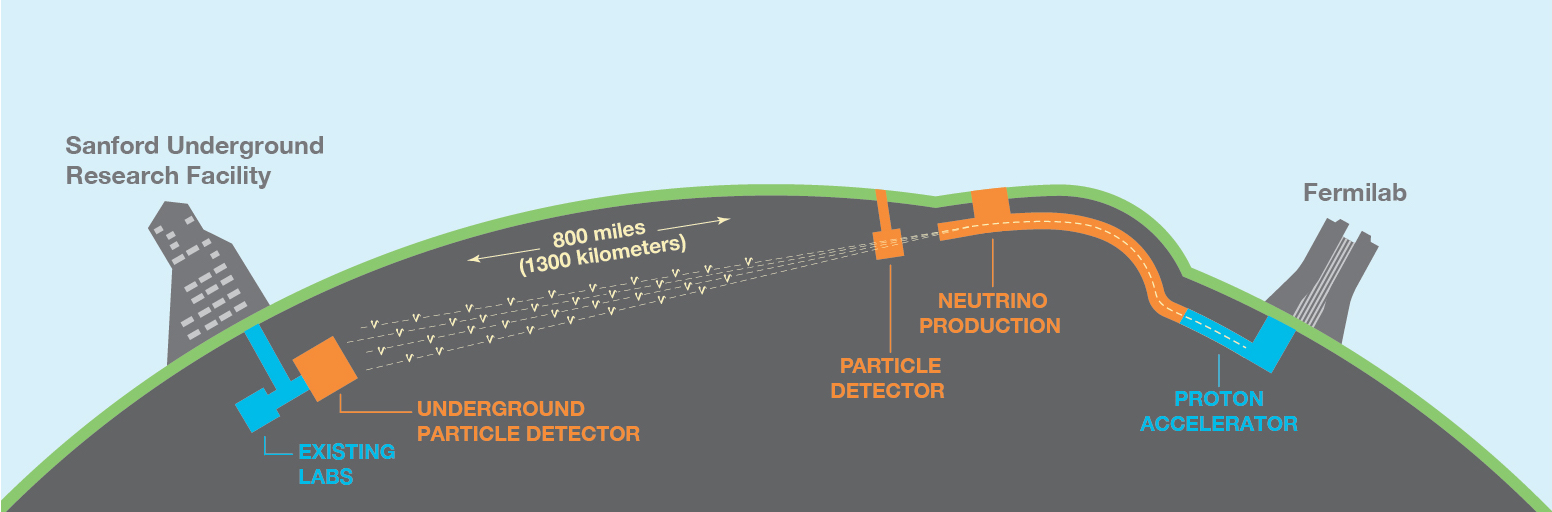
\includegraphics[width=14cm]{DUNE.jpg}
  \caption[Cartoon showing the configuration of the Deep Underground Neutrino Experiment.]{Cartoon showing the configuratuon of the Deep Underground Neutrino Experiment.  The experiment will be based at Fermilab, shown at the right of the figure, and will send neutrinos towards SURF, at the left hand side.  The distance travelled, through the Earth's crust, will be 1300~km.}
  \label{fig:DUNE}
\end{figure}

The DUNE experiment will be discussed in this present chapter.  An overview of the experiment, including its motivation, will be presented in Section \ref{sec:DUNEOverview} before the experimental details are discussed in Section \ref{sec:DUNEExperiment}.  The sensitivities of the experiment and its potential discoveries are the subject of Section \ref{sec:DUNEEffect}.  Finally, the schedule and stategy implemented by the collaboration to ensure commencement of data taking in around ten years' time is outlined in Section \ref{sec:RoadToDUNE}.

%----------------------------------------------------------------------------------------------------------------------------------------------------------------------------
\section{Overview of DUNE}\label{sec:DUNEOverview}

The outstanding questions in neutrino physics discussed in Section \ref{sec:NeutrinoPhysicsStatus}, namely the resolution of the mass hierachy, the determination of the CP-violating phase $\delta_{\textnormal{CP}}$, the measurement of the octant of $\theta_{23}$ and precision calculations of all the mixing angles, motivate the need for next generation experiments.  The DUNE experiment will make decisive contributions to each of these areas; it will also search for nucleon decay with the ability to set world-leading proton lifetime limits and make detailed, unique measurements of the $\nu_e$ flux from a core-collapse supernovae within our galaxy should one occur during the experiment.  Along with this, DUNE will be used to look for Beyond Standard Model physics (such as non-standard interaction and sterile neutrinos), signatures of dark matter and, utilising the capable near detector, measurements of a range of neutrino cross-sections and nuclear effects including final state interations.

The chosen technology for the DUNE far detector, in order to maximise sensitivity to all these factors, is a liquid argon (LAr) TPC (LArTPC), introduced and described in Section \ref{sec:LArTPC}.  The detector will contain four modules, each comprised of 10~kton fiducial LAr and separate data acquisition and readout systems.  The beam will be provided by Fermilab as part of its PIP-II program \cite{} and will be wide band, enabling the study of a range of neutrino energies.  This facilitates a study of multiple oscillation peaks, essentially due to differing $L/E$ ratios, and is relevant when considering the effects of an unknown CP-violating phase and unresolved mass hierarchy.  Since the impact of both of these uncertainties is apparent as an asymmetry between neutrinos and antineutrinos (Equation \ref{eq:NeutrinoAntineutrinoAsymmetry}), there is an implicit degeneracy which must be resolved to ensure both phenomena are correctly determined.  Having access to multiple oscillation peaks means this may be dealt with in a single experiment, as demonstrated in Figure \ref{fig:TwoPeakAmbiguity} \cite{Huber2011}.

\begin{figure}
  \centering
  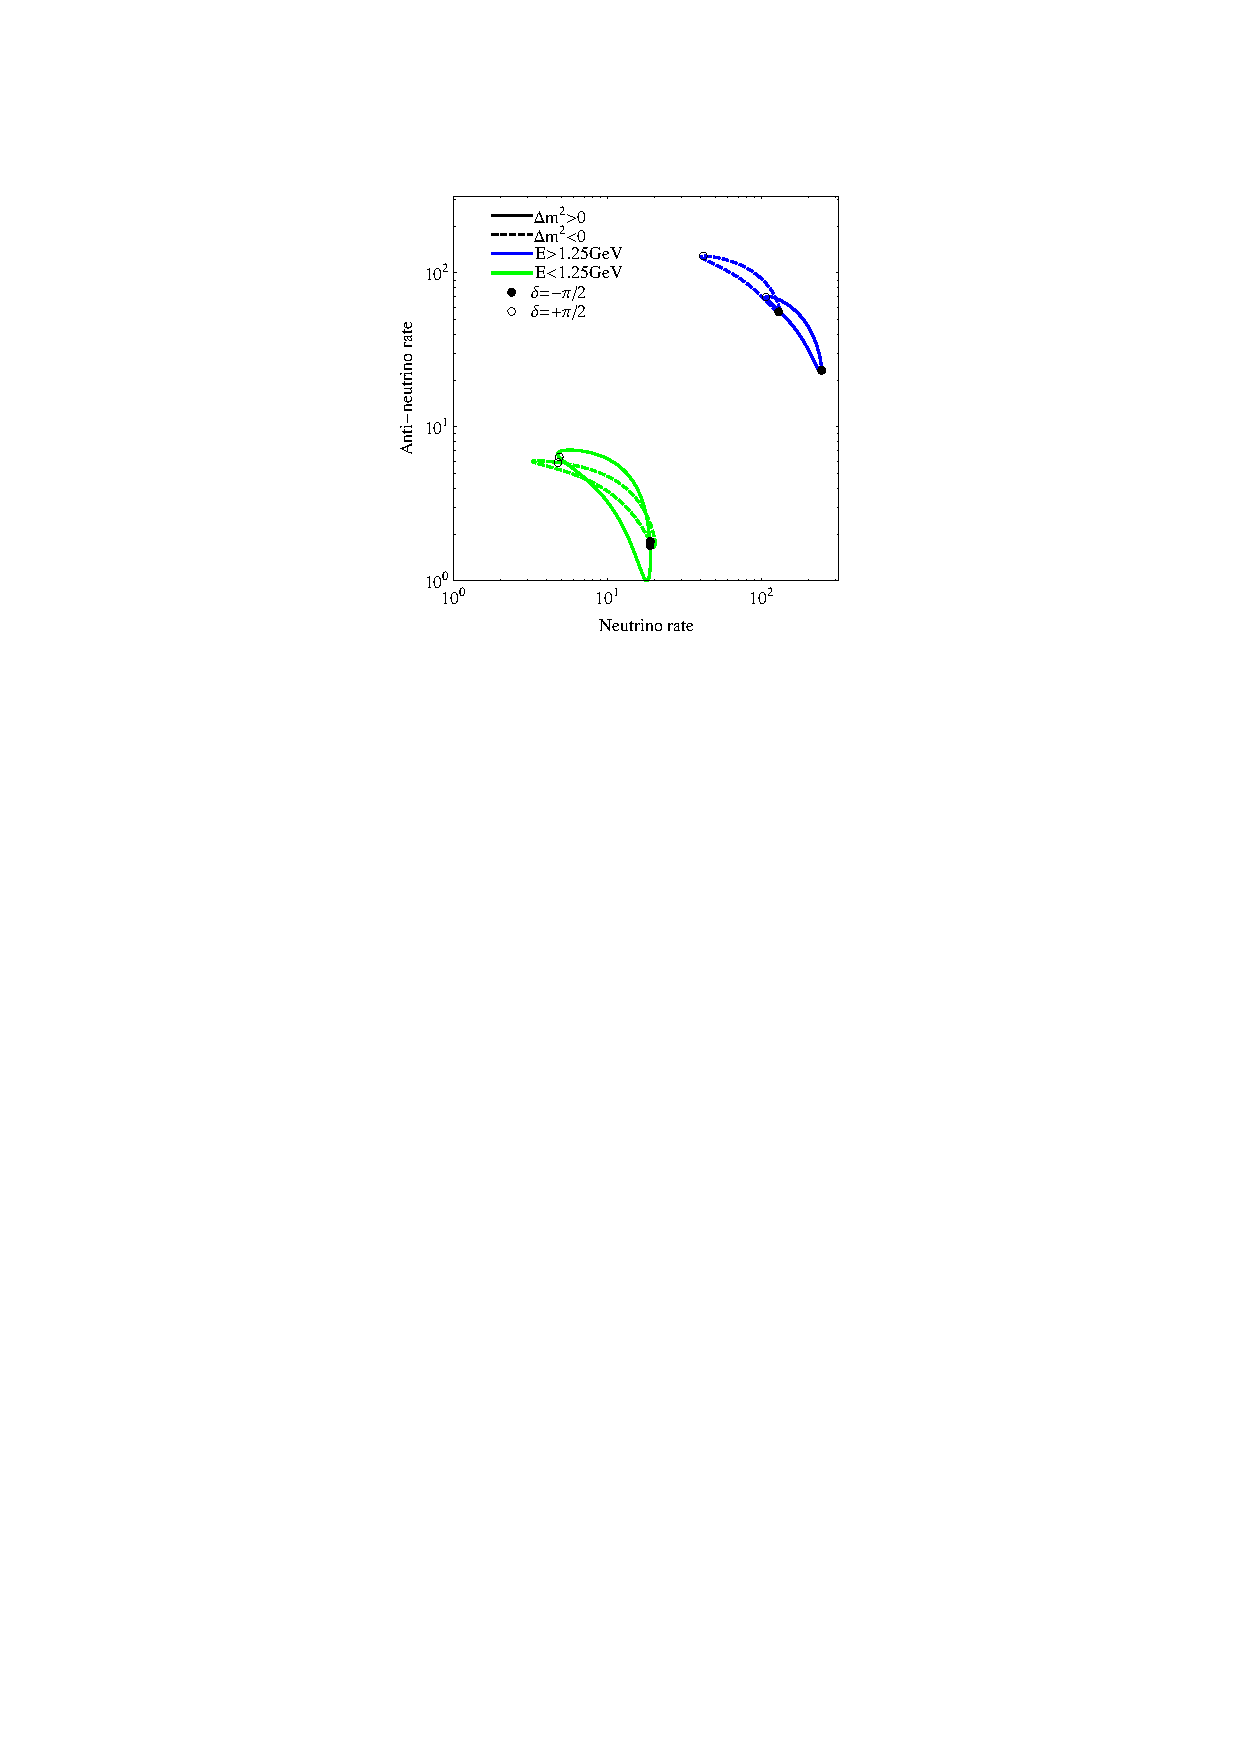
\includegraphics[width=10cm]{TwoPeakAmbiguity.pdf}
  \caption{}
  \label{fig:TwoPeakAmbiguity}
\end{figure}

%----------------------------------------------------------------------------------------------------------------------------------------------------------------------------
\section{Experimental Details}\label{sec:DUNEExperiment}

%----------------------------------------------------------------------------------------------------------------------------------------------------------------------------
\subsection{Beam}\label{sec:DUNEBeam}

%----------------------------------------------------------------------------------------------------------------------------------------------------------------------------
\subsection{Near Detector}\label{sec:NearDetector}

%----------------------------------------------------------------------------------------------------------------------------------------------------------------------------
\subsection{Far Detector}\label{sec:FarDetector}

%----------------------------------------------------------------------------------------------------------------------------------------------------------------------------
\section{The DUNE Effect}\label{sec:DUNEEffect}

%----------------------------------------------------------------------------------------------------------------------------------------------------------------------------
\section{The Road to DUNE}\label{sec:RoadToDUNE}
